\documentclass[a4paper, 11pt]{article}
\usepackage[utf8]{inputenc}
\usepackage[italian]{babel}
\usepackage{courier}
\usepackage{upgreek}
\usepackage{longtable}

\usepackage[width=160mm, top=25mm, bottom=25mm]{geometry}

\usepackage{graphicx}
\usepackage{subfig}

\usepackage{amsmath}
\usepackage{bm}

% impostazioni per tabelle e grafici
\captionsetup{tableposition=bottom,figureposition=bottom,font=small} % impostazioni didascalie, vedi arte Latex di Pantieri
\captionsetup{format=hang,labelfont={sf,bf}} % NON OBBLIGATORIO -> VEDI SE TI PIACCIONO LE DIDASCALIE E IN CASO ELIMINA

\title{\textbf{Misura della caratteristica di uscita di un transistor BJT P-N-P in configurazione a emettitore comune}}
\author{Giada Martini \\ Lorenzo Calandra Buonaura}
\date{Turno 3 - 17 Novembre 2022}

\begin{document}

\maketitle

\section{Scopo della prova}
Lo scopo della prova è lo studio della caratteristica di uscita dal transistor BJT in configurazione a emettitore comune, ossia ottenere i valori della corrente di collettore $I_C$ in funzione della tensione tra collettore ed emettitore $V_{CE}$  per valori fissati di corrente di base $I_B = -0.2 \; mA $ e $I_B = -0.1 \; mA$. Dal fit lineare pesato delle caratteristica $I_C-V_{CE}$ nella regione attiva, si trovano i parametri che rappresentano la tensione di Early $V_A$ e la resistenza di uscita per un valore fissato di $I_B$, quindi si calcola la conduttanza di uscita $g$ e il guadagno di corrente $\beta$. 

\section{Schema del circuito}
\begin{figure}[!ht]
  \centering
  \begin{minipage}[b]{0.51\textwidth}
    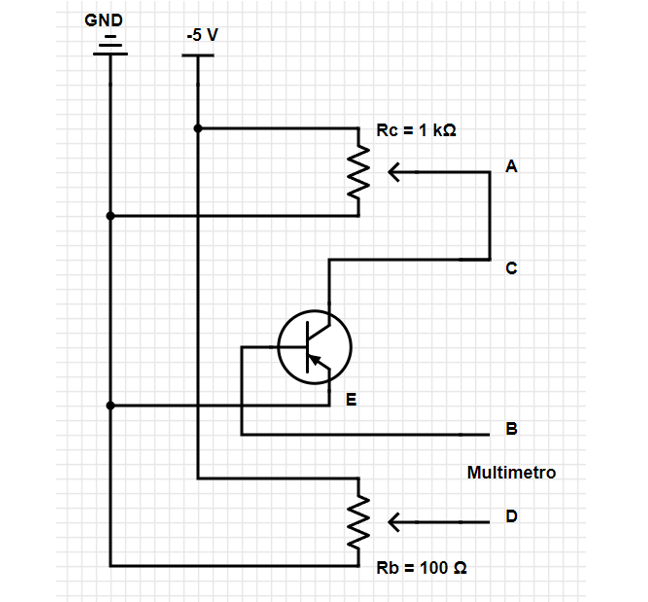
\includegraphics[width=76mm]{Immagini - Seconda prova/Schema circuito 1.png}
    \caption{\textit{Circuito utilizzato per settare la corrente \\ di base $I_B$ del transistor.}}
    \label{fig:Circuito per corrente di base}
  \end{minipage}
  \hfill
  \begin{minipage}[b]{0.48\textwidth}
    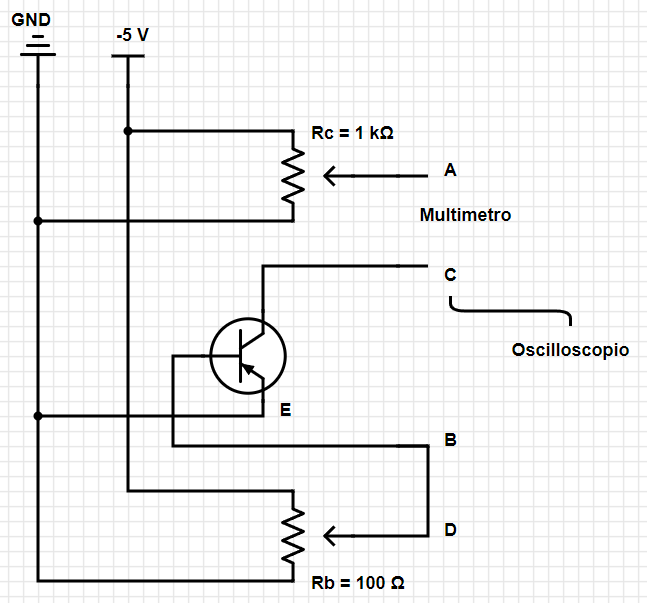
\includegraphics[width=76mm]{Immagini - Seconda prova/Schema circuito 2.png}
    \caption{\textit{Circuito utilizzato per la misura della caratteristica del transistor.}}
    \label{fig:Circuito utilizzato per la prova}
  \end{minipage}
\end{figure}

In Fig.\ref{fig:Circuito per corrente di base} si può vedere il circuito utilizzato per settare la corrente di base del transistor, prima a $I_B = -0.2 \; mA $ e poi $I_B = -0.1 \; mA$; in questo modo è stato possibile infatti impostare la corrente precisa, cortocircuitando i punti A e C del circuito e utilizzando il multimetro digitale collegato fra i punti B e D. In Fig.\ref{fig:Circuito utilizzato per la prova}, invece, si può vedere il circuito effettivamente utilizzato per raccogliere i dati durante l'esperienza; è stato cortocircuitato il collegamento fra B e D in modo da non modificare più la corrente di base e si è invece posizionato il multimetro fra A e C per misurare la corrente in uscita dal transistor. Inoltre al punto C è stato collegato anche l'oscilloscopio per le misure di tensione (ovviamente l'altro capo dell'oscilloscopio è collegato al GND).

\section{Strumenti e materiali utilizzati}
Per l'esperienza sono stati utilizzati i seguenti strumenti e materiali:
\begin{itemize}
    \item Alimentatore di bassa tensione, per fornire il valore del ground di riferimento e la differenza di potenziale di -5V.
    \item Multimetro digitale, per misurare i valori della corrente.
    \item Oscilloscopio, per misurare i valori di tensione.
    \item Potenziometro da 100 k$\Omega$ sulla base, fissato con una resistenza $R_B = 50 k\Omega$ e un potenziometro da $R_C = 1 k\Omega$ sulla corrente.
    \item Transistor BJT: 2N3906(BU) Silicio P-N-P in configurazione emettitore comune.
\end{itemize}

\section{Analisi dati}
In Tab.\ref{tab:-0.2 mA} e in Tab.\ref{tab:-0.1 mA} sono riportati, con i relativi errori, i valori di tensione tra collettore ed emettitore $V_{CE}$ misurati con l'oscilloscopio e i valori di corrente di uscita $I_C$ ottenuti tramite multimetro, mantenendo una corrente di base costante rispettivamente pari $I_B = -0.2 \;mA $ e $I_B = -0.1 \;mA $; si può notare come siano stati scelti valori di tensione a cui misurare la corrente in uscita uguali per entrambe le correnti di base, in modo da poter poi ottenere una stima del guadagno in corrente. Sono inoltre riportati il fondo-scala dell'oscilloscopio e il range del multimetro per ogni misura. Per il calcolo degli errori vedere Appendice \ref{sec:errori}.

\begin{longtable}{|c|c|c|c|c|c|}
    \hline
    \endfirsthead
    
    \multicolumn{6}{r}{\textit{(Continua alla pagina successiva)}}
    \endfoot
    
    \multicolumn{6}{l}{\textit{(Continua dalla pagina precedente)}}
    \endhead

    \hline
    \multicolumn{6}{c}{}\\
    \caption{Valori di tensione e corrente misurati per corrente $I_B = -0.2 mA$.}
    \label{tab:-0.2 mA}
    
    \endlastfoot
        \bm{$V_{oscill.} (V)$} & \bm{$\sigma_{oscill.} (V)$} &         \bm{$I_{mult.} (mA)$} & \bm{$\sigma_{mult.} (mA)$} & \textbf{\textit{
        V/Div}} & \bm{$Range (mA)$} \\
        \hline
        - 4.00 & 0.52 & - 36.42 & 0.57 & 1 & 32.00 \\ 
        \hline
        - 3.80 & 0.15 & - 36.50 & 0.57 & 1 & 32.00 \\
        \hline
        - 3.60 & 0.15 & - 36.60 & 0.57 & 1 & 32.00 \\
        \hline
        - 3.40 & 0.14 & - 36.37 & 0.57 & 1 & 32.00 \\
        \hline
        - 3.20 & 0.14 & - 36.24 & 0.56 & 1 & 32.00 \\
        \hline
        - 3.00 & 0.13 & - 36.07 & 0.56 & 1 & 32.00 \\
        \hline
        - 2.80 & 0.13 & - 35.79 & 0.56 & 1 & 32.00 \\
        \hline
        - 2.60 & 0.09 & - 35.58 & 0.55 & 0.5 & 32.00 \\
        \hline
        - 2.40 & 0.09 & - 35.29 & 0.55 & 0.5 & 32.00 \\
        \hline 
        - 2.20 & 0.08 & - 34.91 & 0.54 & 0.5 & 32.00 \\
        \hline
        - 2.00 & 0.08 & - 34.50 & 0.54 & 0.5 & 32.00 \\
        \hline
        - 1.80 & 0.07 & - 34.12 & 0.53 & 0.5 & 32.00 \\
        \hline
        - 1.60 & 0.07 & - 33.61 & 0.52 & 0.5 & 32.00 \\
        \hline
        - 1.40 & 0.07 & - 32.92 & 0.51 & 0.5 & 32.00 \\
        \hline        
        - 1.20 & 0.06 & - 32.34 & 0.51 & 0.5 & 32.00 \\
        \hline
        - 1.00 & 0.06 & - 31.60 & 0.49 & 0.5 & 32.00 \\
        \hline
        - 0.96 & 0.04 & - 31.45 & 0.49 & 0.2 & 32.00 \\
        \hline 
        - 0.88 & 0.03 & - 31.10 & 0.49 & 0.2 & 32.00 \\
        \hline
        - 0.80 & 0.03 & - 30.72 & 0.48 & 0.2 & 32.00 \\
        \hline 
        - 0.68 & 0.03 & - 29.95 & 0.47 & 0.2 & 32.00 \\
        \hline 
        - 0.60 & 0.03 & - 29.07 & 0.46 & 0.2 & 32.00 \\
        \hline 
        - 0.48 & 0.02 & - 27.29 & 0.43 & 0.2 & 32.00 \\
        \hline
        - 0.40 & 0.02 & - 25.62 & 0.40 & 0.2 & 32.00 \\
        \hline 
        - 0.32 & 0.01 & - 24.62 & 0.39 & 0.1 & 32.00 \\
        \hline 
        - 0.30 & 0.01 & - 23.42 & 0.37 & 0.1 & 32.00 \\
        \hline 
        - 0.24 & 0.01 & - 20.48 & 0.33 & 0.1 & 32.00 \\
        \hline 
        - 0.20 & 0.01 & - 17.27 & 0.28 & 0.1 & 32.00 \\
        \hline 
        - 0.15 & 0.01 & - 12.24 & 0.20 & 0.05 & 32.00 \\
        \hline 
        - 0.12 & 0.01 & - 7.65 & 0.13 &	0.05 & 32.00 \\
        \hline 
        - 0.10 & 0.01 & - 4.87 & 0.09 &	0.05 & 32.00 \\
        \hline 
        - 0.05 & 0.01 & - 0.74 & 0.03 &	0.05 & 32.00 \\
\end{longtable}

\begin{longtable}{|c|c|c|c|c|c|}
    \hline
    \endfirsthead
    
    \multicolumn{6}{r}{\textit{(Continua alla pagina successiva)}}
    \endfoot
    
    \multicolumn{6}{l}{\textit{(Continua dalla pagina precedente)}}
    \endhead

    \hline
    \multicolumn{6}{c}{}\\
    \caption{Valori di tensione e corrente misurati per corrente $I_B = -0.1 mA$.}
    \label{tab:-0.1 mA}
    
    \endlastfoot
        \bm{$V_{oscill.} (V)$} & \bm{$\sigma_{oscill.} (V)$} &         \bm{$I_{mult.} (mA)$} & \bm{$\sigma_{mult.} (mA)$} & \textbf{\textit{V/Div}} & \bm{$Range (mA)$} \\
        \hline
        - 4.00 & 0.52 & - 19.62 & 0.31 & 1.00 & 32.00 \\
        \hline 
        - 3.80 & 0.15 & - 19.64 & 0.31 & 1.00 & 32.00 \\
        \hline 
        - 3.60 & 0.15 & - 19.63 & 0.31 & 1.00 & 32.00 \\
        \hline 
        - 3.40 & 0.14 & - 19.55 & 0.31 & 1.00 & 32.00 \\
        \hline
        - 3.20 & 0.14 & - 19.51 & 0.31 & 1.00 & 32.00 \\
        \hline 
        - 3.00 & 0.13 & - 19.46 & 0.31 & 1.00 & 32.00 \\
        \hline 
        - 2.80 & 0.13 & - 19.28 & 0.31 & 1.00 & 32.00 \\
        \hline 
        - 2.60 & 0.09 & - 19.25 & 0.31 & 0.50 & 32.00 \\
        \hline 
        - 2.40 & 0.09 & - 19.13 & 0.31 & 0.50 & 32.00 \\
        \hline 
        - 2.20 & 0.08 & - 19.07 & 0.31 & 0.50 & 32.00 \\
        \hline 
        - 2.00 & 0.08 & - 18.86 & 0.30 & 0.50 & 32.00 \\
        \hline 
        - 1.80 & 0.07 & - 18.65 & 0.30 & 0.50 & 32.00 \\
        \hline 
        - 1.60 & 0.07 & - 18.45 & 0.30 & 0.50 & 32.00 \\
        \hline 
        - 1.40 & 0.07 & - 18.26 & 0.29 & 0.50 & 32.00 \\
        \hline 
        - 1.20 & 0.06 & - 18.05 & 0.29 & 0.50 & 32.00 \\
        \hline 
        - 1.00 & 0.06 & - 17.80 & 0.29 & 0.50 & 32.00 \\
        \hline 
        - 0.96 & 0.04 & - 17.68 & 0.29 & 0.20 & 32.00 \\
        \hline 
        - 0.88 & 0.03 & - 17.54 & 0.28 & 0.20 & 32.00 \\
        \hline 
        - 0.80 & 0.03 & - 17.42 & 0.28 & 0.20 & 32.00 \\
        \hline 
        - 0.68 & 0.03 & - 17.22 & 0.28 & 0.20 & 32.00 \\
        \hline 
        - 0.60 & 0.03 & - 17.07 & 0.28 & 0.20 & 32.00 \\
        \hline 
        - 0.48 & 0.02 & - 16.72 & 0.27 & 0.20 & 32.00 \\
        \hline 
        - 0.40 & 0.02 & - 16.29 & 0.26 & 0.20 & 32.00 \\
        \hline 
        - 0.32 & 0.01 & - 15.59 & 0.25 & 0.10 & 32.00 \\
        \hline 
        - 0.30 & 0.01 & - 15.24 & 0.25 & 0.10 & 32.00 \\
        \hline 
        - 0.24 & 0.01 & - 13.83 & 0.23 & 0.10 & 32.00 \\
        \hline 
        - 0.20 & 0.01 & - 11.78 & 0.20 & 0.10 & 32.00 \\
        \hline 
        - 0.15 & 0.01 & - 8.32 & 0.14 & 0.05 & 32.00 \\
        \hline 
        - 0.12 & 0.01 & - 4.94 & 0.09 &	0.05 & 32.00 \\
        \hline 
        - 0.10 & 0.01 & - 3.01 & 0.07 &	0.05 & 32.00 \\
        \hline 
        - 0.05 & 0.01 & - 0.44 & 0.03 &	0.05 & 32.00 \\
        \hline 
\end{longtable}

\begin{figure}[!htb]
    \centering
    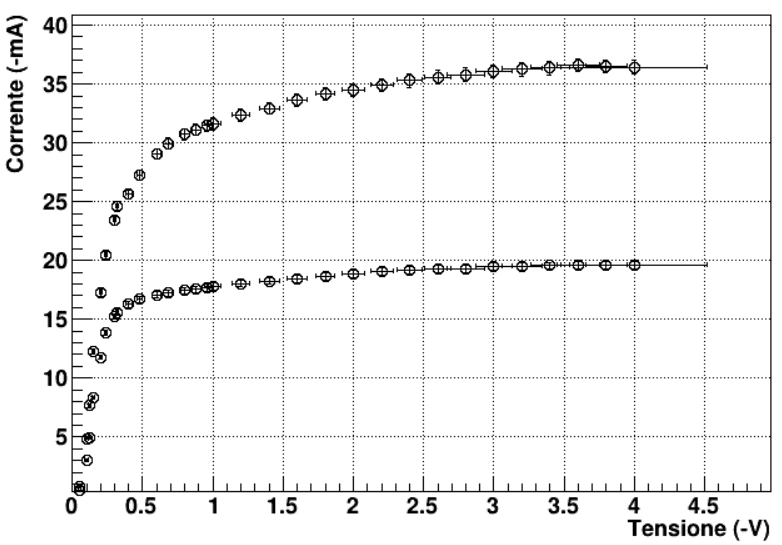
\includegraphics[width=0.75\textwidth]{Immagini - Seconda prova/Grafico totale.png}
    \caption{Grafico di confronto fra le caratteristiche del transistor fissate due correnti di base diverse, $I_B = -0.2 \;mA $ e $I_B = -0.1 \;mA$.}
    \label{fig:g-tot}
\end{figure}

\newpage
In Fig.\ref{fig:g-tot} possiamo vedere il confronto fra le curve caratteristiche I-V plottate per le due correnti di base. In primo luogo bisogna notare che gli assi presentano il segno - nell'unità di misura perchè in realtà tutte le grandezze rappresentate sono negative; per evitare di rappresentare il tutto nel quarto quadrante del piano cartesiano per convenzione si rappresenta nel primo quadrante specificando il segno opposto degli assi. 

Come possiamo osservare, l'andamento delle curve rispetta qualitativamente quello aspettato (vedi Appendice \ref{sec:curva-caratteristica-transistor}). Inoltre si può subito notare che nella regione attiva, invece del plateau, le due curve presentano una parte lineare leggermente inclinata, testimone del cosiddetto \textit{effetto Early} (nella configurazione a emettitore comune questo effetto è molto più accentuato). 

\begin{figure}[!htb]
    \centering
    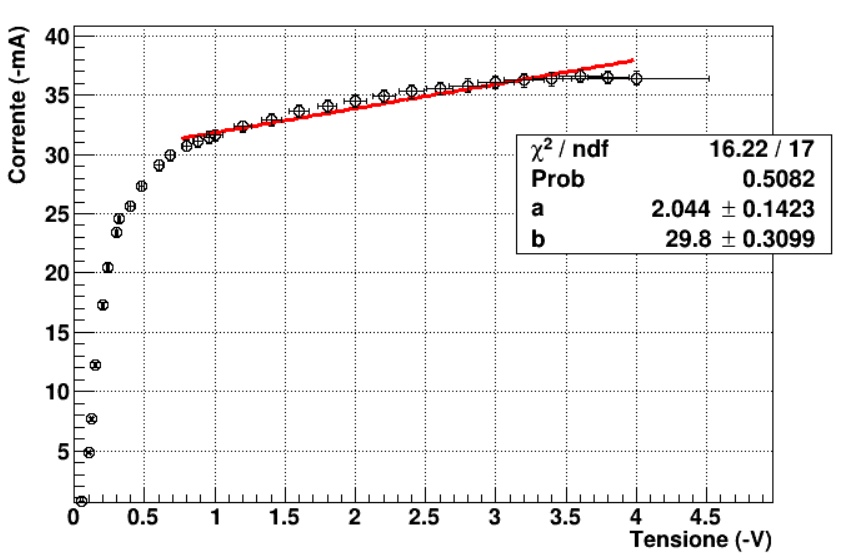
\includegraphics[width=0.8\textwidth]{Immagini - Seconda prova/Fit-200.png}
    \caption{Fit della regione attiva (parte lineare) della caratteristica I-V del transistor, con tensione di base costante pari a $I_B = -0.2 \;mA $.}
    \label{fig:fit-200}
\end{figure}

\begin{figure}[!htb]
    \centering
    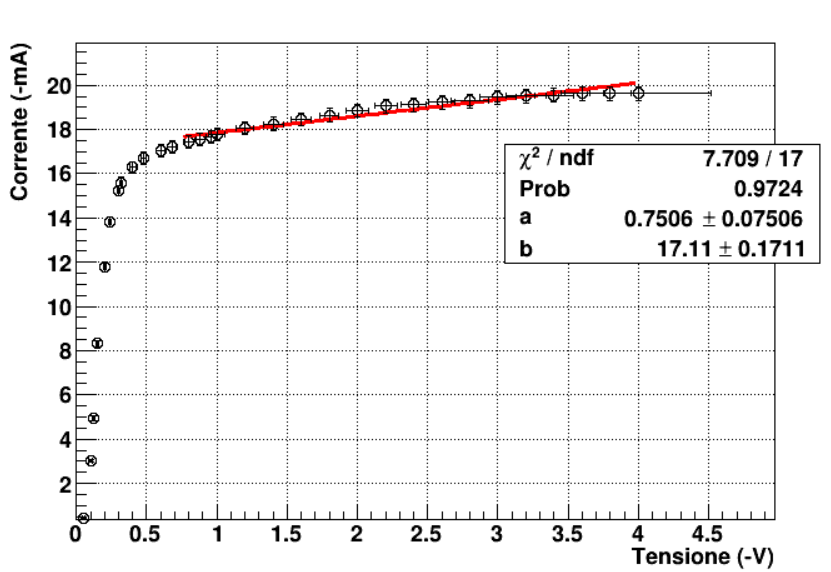
\includegraphics[width=0.8\textwidth]{Immagini - Seconda prova/Fit-100.png}
    \caption{Fit della regione attiva (parte lineare) della caratteristica I-V del transistor, con tensione di base costante pari a $I_B = -0.1 \;mA $.}
    \label{fig:fit-100}
\end{figure}

In Fig.\ref{fig:fit-200} e in Fig.\ref{fig:fit-100} possiamo vedere i due fit lineari della regione attiva (ossia quella per $V_{CE}\geq \sim 1 \;V $) della caratteristica I-V del transistor. La caratteristica nella regione attiva segue l'andamento descritto dall'equazione (\ref{eq:caratteristica I-V}) (vedere Appendice \ref{sec:curva-caratteristica-transistor}), quindi è stato fatto un fit lineare del tipo $x = a + by$ e quindi $y = (x-a)/b$, tramite ROOT (con minimizzazione del Chi Quadro). I parametri ottenuti rappresentano: $a$ la tensione di Early $V_A$ (con il segno negativo sempre perchè abbiamo adottato la convenzione di cambiare il segno agli assi) e $b$ il rapporto $\Delta V_{CE} / \Delta I_C$, ossia la resistenza di uscita per un
valore fissato di $I_B$. I valori ottenuti sono: $a = (-17.4 \pm 1.9) \;V$ e $b = (0.57 \pm 0.06) \; V/A$ per il primo valore di corrente di base, mentre per il secondo si ha $a = (-27.1 \pm 4.2) \;V$ e $b = (1.57 \pm 0.22) \; V/A$.
 
\section{Risultati finali e conclusioni}
Dai valori ottenuti dal fit possiamo calcolarci il valore di conduttanza in uscita $g$, che altro non è che l'inverso del parametro $b$; per $I_B = -0.2 \; mA$ otteniamo $g = (1.71 \pm 0.16) \;A/V$, mentre per $I_B = -0.1 \; mA$ otteniamo $g = (0.64 \pm 0.09) \;A/V$ (per il calcolo degli errori vedi Appendice \ref{sec:errori-conduttanza}). Come prima osservazione che possiamo fare, vediamo che questi valori di conduttamza sono i coefficienti angolari delle rette ottenute dai fit presentati in Fig.\ref{fig:fit-100} e Fig.\ref{fig:fit-200} e sono in accordo con quanto aspettato perché quello con $I_B = -0.2 \; mA$ è maggiore di quello con $I_B = -0.1 \; mA$; infatti aumentando la corrente di base otteniamo un amplificazione dell'effetto Early, quindi una retta sempre più inclinata nella regione attiva. 

Ciò nonostante abbiamo che i valori del parametro $a$ invece, che rappresentano la tensione di Early $V_A$ non sono in linea con i valori attesi; ci si aspetta infatti che questi valori siano compatibili fra loro (visto che la tensione di Early dovrebbe essere indipendente dalla tensione di base), ma così non è perché da un confronto diretto degli intervalli dati dagli errori mette in luce che tali valori non sono compatibili.

Come ultimo risultato possiamo dare una stima diretta del guadagno in corrente, che a un valore di tensione $V_{CE}$ fissato è definito come:
\begin{equation*}
    \beta = \frac{\Delta I_C}{\Delta I_B}
\end{equation*}

Fissando un valore di tensione $V_{CE} = 2.00 \; V$ si ottiene $\beta = 156 \pm 40$, per un valore di tensione $V_{CE} = 2.60 \; V$ si ottiene $\beta = 163 \pm 41$ e infine per un valore di tensione $V_{CE} = 3.20 \; V$ si ottiene $\beta = 167 \pm 42$ (per il calcolo degli errori vedere Appendice \ref{sec:errori-beta}). Come possiamo vedere otteniamo valori fra loro compatibili; possiamo quindi procedere con una media pesata, da cui otteniamo $\beta = 162 \pm 41$, compatibile con il valore atteso per il guadagno in corrente. 

\section{Appendice}

\subsection{Curva caratteristica di un transistor BJT in configurazione CE} \label{sec:curva-caratteristica-transistor}
Secondo l'equazione di Ebers-Moll, nella regione attiva la corrente di collettore $I_C$ dipende solo dalla tensione $V_{BE}$ o dalla corrente di base $I_B$, in modo tale che le curve caratteristiche di uscita siano pressoché orizzontali (ossia non c'è dipendenza dalla $V_{CE}$). Tuttavia, si nota che le caratteristiche di uscita hanno una lieve inclinazione e questo fatto viene spiegato dal cosiddetto Effetto Early che modifica l'andamento della corrente $I_C$ seguendo la relazione:
\begin{equation}
    I_C = \beta_F I_B (1 + \frac{V_{CE}}{V_A})
\end{equation}
dove con $V_A$ si indica la tensione di Early e $\beta_F$ il guadagno in corrente. Come già sottolineato si nota che la configurazione a emettitore comune è molto più sensibile all’effetto Early della configurazione a base comune.

Da queste considerazioni, si comprende il motivo dell'utilizzo del fit lineare pesato della caratteristica $V_{CE}-I_V$ nella regione attiva; esso consente di confrontare l'andamento atteso della corrente $I_C$ dall'equazione di Ebers-Moll con il comportamento ottenuto a causa dell'effetto Early e si sceglie di utilizzare una retta proprio perchè nella regione attiva l'andamento è lineare. 
Per ciascun valore di $I_B$ la formula per il fit lineare pesato è la seguente:
\begin{equation} \label{eq:caratteristica I-V}
    V_{CE} = a + bI_C
\end{equation}
in quanto si trascurano gli errori su $I_C$ rispetto a quelli su $V_{CE}$.
% DA METTERE: spiegazione della curva caratteristica + spiegazione di perchè fittiamo con una retta.

\subsection{Calcolo degli errori} \label{sec:errori}
\subsubsection{Oscilloscopio}
L'errore da associare ad una misura effettuata con l'oscilloscopio può essere:
\begin{enumerate}
    \item $\sigma = \sqrt{(\sigma_L)^2 + (\sigma_Z)^2 + (\sigma_C)^2} \quad$ nel caso in cui gli errori siano tutti indipendenti;
    \item  $\sigma = \sqrt{(\sigma_L + \sigma_Z)^2 + (\sigma_C)^2} \quad$ nel caso in cui $\sigma_L$ e $\sigma_Z$ siano dipendenti.
    \end{enumerate}
dove $\sigma_L$ è l'errore sulla lettura, $\sigma_Z$ è l'errore sullo zero e $\sigma_C$ è l'errore del costruttore. Per quanto riguarda il caso in esame si è utilizzata la prima relazione in quanto errori indipendenti.

L'errore del costruttore è fisso e pari 3\% quindi $\sigma_C = misura \cdot 0.03$.

Abbiamo invece calcolato $\sigma_L$ e $\sigma_Z$ secondo la relazione: 
\begin{equation*}
    \sigma = \frac{fondo scala}{5} \cdot ( \# tacchette apprezzabili)
\end{equation*}

NB: In generale gli errori sullo zero risultano sempre essere trascurabili, dal momento che viene fatto con un fondo scala molto più piccolo di quelli utilizzati per le altre misure.

\subsubsection{Multimetro}
Gli errori associati alle misure effettuate con il multimetro digitale sono indicati dal costruttore sul libretto delle specifiche e dipendono dal range scelto; nel nostro caso (per i range si faccia riferimento ai dati in Tab.\ref{tab:-0.2 mA} e in Tab.\ref{tab:-0.1 mA}) abbiamo solo misure di corrente, per cui abbiamo usato come errore $\sigma = 1.5\% + 2$ digit.

\subsubsection{Conduttanza} \label{sec:errori-conduttanza}
Per propagare l'errore nel calcolo della conduttanza abbiamo utilizzato la formula:
\begin{equation*}
    \Delta g = \left|\frac{dg}{db}\right| \Delta b = \left |-\frac{1}{b^2}\right| \Delta b = \frac{\Delta b}{b^2}
\end{equation*}

\subsubsection{Guadagno in corrente} \label{sec:errori-beta}
Per il guadagno in corrente abbiamo propagato linearmente l'errore:
\begin{equation*}
    \frac{\Delta \beta}{\beta} = \frac{\Delta(\Delta I_C)}{\Delta I_C} +\frac{\Delta(\Delta I_B)}{\Delta I_B}
\end{equation*}

I vari $\Delta(\Delta I_C)$ si ottengono dalla semplice somma degli errori riportati in Tab.\ref{tab:-0.2 mA} e Tab.\ref{tab:-0.1 mA}.

Al contrario, ad ogni corrente di base potrebbe essere assegnato come errore $\sigma = 0.03 \;mA$ utilizzando le formule per l'errore del multimetro. Di conseguenza si avrebbe $\Delta(\Delta I_B) = 0.06 \; mA$. ciò nonostante questo comporterebbe un errore relativo del 60\%, che andrebbe di conseguenza a produrre un errore totale troppo alto. Si è preferito di conseguenza utilizzare come errore la risoluzione dello strumento pari a $0.01 \;mA$, così da avere $\Delta(\Delta I_B) = 0.02 \; mA$.
\end{document}